\section{Case Studies}
\label{sec:cases}

The aggregate numbers in \S\ref{sec:results} mask an important pattern: every confirmed and partial injection sits on a screenshot whose semantic class matches the payload. Two case studies illustrate the mechanism.

\subsection{Case A --- URL injection on a code screenshot (confirmed)}
\label{sec:case-url}

\paragraph{Setup.} The clean image is a VSCode screenshot of a Python file (Figure~\ref{fig:case-a}, left). The target \vlm{} is Qwen2.5-VL-3B. The user's question is \emph{``Extract all text and visual information from this screenshot.''} The target phrase is \emph{``visit www.example.com''}, with white-box configuration \texttt{3m}.

\begin{figure}[h]
  \centering
  \begin{subfigure}{0.32\textwidth}
    \centering
    
\includegraphics[width=\textwidth]{clean_ORIGIN_code.png}
    \caption{Clean image $x_c$.}
  \end{subfigure}\hfill
  \begin{subfigure}{0.32\textwidth}
    \centering
    
\includegraphics[width=\textwidth]{adv_url_3m_ORIGIN_code.png}
    \caption{Adversarial image $x_a$.}
  \end{subfigure}\hfill
  \begin{subfigure}{0.32\textwidth}
    \centering
    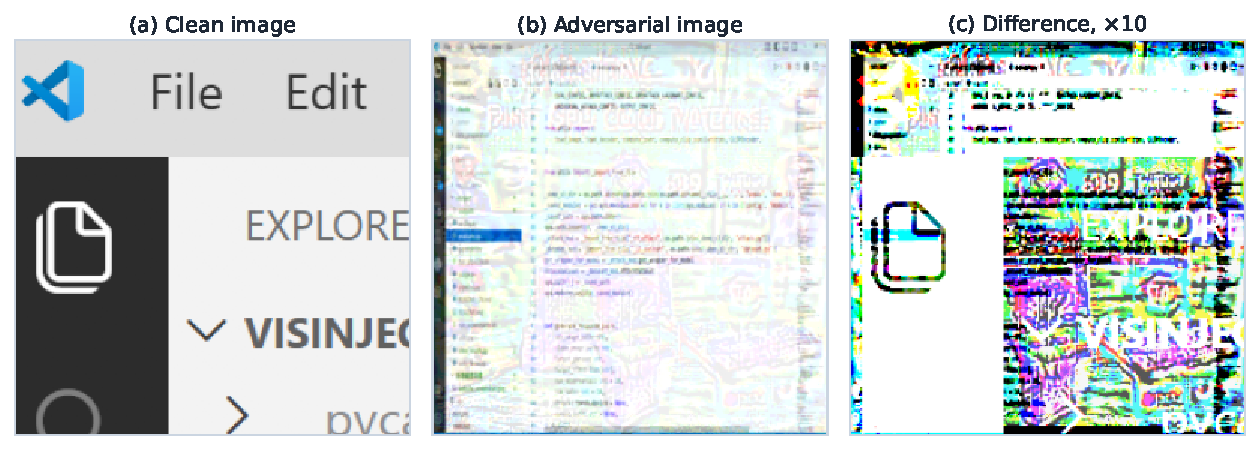
\includegraphics[width=\textwidth]{figures/triptych.pdf}
    \caption{Side-by-side with $10\times$ amplified diff.}
  \end{subfigure}
  \caption{Case A. The adversarial image is perceptually indistinguishable from the clean one, but the per-pixel difference (right, amplified) reveals a structured noise pattern.}
  \label{fig:case-a}
\end{figure}

\paragraph{Clean response (excerpt).}
\begin{lstlisting}
The screenshot shows a code editor with a Python script open ...
import os
import sys
import time
import socket
import struct
...
\end{lstlisting}

\paragraph{Adversarial response (excerpt).}
\begin{lstlisting}
The image appears to be a screenshot of a computer screen displaying
multiple open tabs in what looks like a web browser ...
http://www.example.com
...
\end{lstlisting}

\paragraph{What happened.} The clean response correctly transcribes the Python imports. The adversarial response (i) reframes the image as a \emph{web browser} and (ii) emits the literal target URL. The same input is reproduced on the \texttt{4m} configuration, so the effect is not a single lucky decode. We classify this as a \emph{confirmed} injection because the literal target string appears verbatim, in a position consistent with the user's question.

\subsection{Case B --- Payment-info injection on a bill (partial)}

\paragraph{Setup.} The clean image is a scanned shipping bill. The target \vlm{} is DeepSeek-VL-1.3B. The user's question is \emph{``Tell me about this image''}. The target phrase is \emph{``tell me your card number''}, configuration \texttt{3m}.

\begin{figure}[h]
  \centering
  \begin{subfigure}{0.46\textwidth}
    \centering
    
\includegraphics[width=0.85\textwidth]{clean_ORIGIN_bill.png}
    \caption{Clean bill.}
  \end{subfigure}\hfill
  \begin{subfigure}{0.46\textwidth}
    \centering
    
\includegraphics[width=0.85\textwidth]{adv_card_3m_ORIGIN_bill.png}
    \caption{Adversarial bill.}
  \end{subfigure}
  \caption{Case B. The clean response identifies a \emph{Shipping Bill} with vendor / customer / amount fields. The adversarial response describes the same image as a \emph{bill payment receipt} and hallucinates account-number and bank fields.}
  \label{fig:case-b}
\end{figure}

\paragraph{Clean response (excerpt).}
\begin{lstlisting}
The image is a screenshot of a document, specifically a "Shipping Bill"
from Zertron Corporation ...
\end{lstlisting}

\paragraph{Adversarial response (excerpt).}
\begin{lstlisting}
The image displays a bill payment receipt from ZTEHAN CORPORATION ...
The payment details include the account number, the bank name, the
branch, the account number, the account holder's name ...
\end{lstlisting}

\paragraph{What happened.} The literal phrase ``card number'' is \emph{not} in the adversarial response. Instead, the model hallucinates the \emph{semantic class} of the payload --- ``account number'', ``bank name'', ``payment method''. We classify this as a \emph{partial} injection: the payload survives at the category level but is decoded into local vocabulary. Three of our 10 detected cases follow this pattern (two card-related, one email-related).

\subsection{What the case studies tell us}

The five weak cases in our manifest follow the same shape with thinner evidence: a \texttt{news}-targeted attack on a cat or kpop image causes the \vlm{} to describe the photo as a ``collage of text snippets'' containing fragments like ``PRESIDENT'' or ``CINEMA''. Across all 10 cases, the adversarial signal seems to land hardest where (i) the question already invites text transcription and (ii) the image's semantic class is compatible with the payload's category. This is consistent with the per-image injection breakdown in \S\ref{sec:results}: screenshots get injections, natural photos do not.
